% -*- Mode:TeX -*-

%% IMPORTANT: The official thesis specifications are available at:
%%            http://libraries.mit.edu/archives/thesis-specs/
%%
%%            Please verify your thesis' formatting and copyright
%%            assignment before submission.  If you notice any
%%            discrepancies between these templates and the 
%%            MIT Libraries' specs, please let us know
%%            by e-mailing thesis@mit.edu

%% The documentclass options along with the pagestyle can be used to generate
%% a technical report, a draft copy, or a regular thesis.  You may need to
%% re-specify the pagestyle after you \include  cover.tex.  For more
%% information, see the first few lines of mitthesis.cls. 

%\documentclass[12pt,vi,twoside]{mitthesis}
%%
%%  If you want your thesis copyright to you instead of MIT, use the
%%  ``vi'' option, as above.
%%
%\documentclass[12pt,twoside,leftblank]{mitthesis}
%%
%% If you want blank pages before new chapters to be labelled ``This
%% Page Intentionally Left Blank'', use the ``leftblank'' option, as
%% above. 

\documentclass[12pt,twoside]{mitthesis}
\usepackage{lgrind}
%% These have been added at the request of the MIT Libraries, because
%% some PDF conversions mess up the ligatures.  -LB, 1/22/2014
\usepackage{cmap}
\usepackage[T1]{fontenc}
%% Package "lmodern" added by user request see ServiceNow INC0396734 -OT, 4/29/2020
\usepackage{lmodern}
\pagestyle{plain}

%% This bit allows you to either specify only the files which you wish to
%% process, or `all' to process all files which you \include.
%% Krishna Sethuraman (1990).

%% \typein [\files]{Enter file names to process, (chap1,chap2 ...), or `all' to
%% process all files:}
%% \def\all{all}
%% \ifx\files\all \typeout{Including all files.} \else \typeout{Including only \files.} \includeonly{\files} \fi

\begin{document}

% -*-latex-*-
% 
% For questions, comments, concerns or complaints:
% thesis@mit.edu
% 
%
% $Log: cover.tex,v $
% Revision 1.8  2008/05/13 15:02:15  jdreed
% Degree month is June, not May.  Added note about prevdegrees.
% Arthur Smith's title updated
%
% Revision 1.7  2001/02/08 18:53:16  boojum
% changed some \newpages to \cleardoublepages
%
% Revision 1.6  1999/10/21 14:49:31  boojum
% changed comment referring to documentstyle
%
% Revision 1.5  1999/10/21 14:39:04  boojum
% *** empty log message ***
%
% Revision 1.4  1997/04/18  17:54:10  othomas
% added page numbers on abstract and cover, and made 1 abstract
% page the default rather than 2.  (anne hunter tells me this
% is the new institute standard.)
%
% Revision 1.4  1997/04/18  17:54:10  othomas
% added page numbers on abstract and cover, and made 1 abstract
% page the default rather than 2.  (anne hunter tells me this
% is the new institute standard.)
%
% Revision 1.3  93/05/17  17:06:29  starflt
% Added acknowledgements section (suggested by tompalka)
% 
% Revision 1.2  92/04/22  13:13:13  epeisach
% Fixes for 1991 course 6 requirements
% Phrase "and to grant others the right to do so" has been added to 
% permission clause
% Second copy of abstract is not counted as separate pages so numbering works
% out
% 
% Revision 1.1  92/04/22  13:08:20  epeisach

% NOTE:
% These templates make an effort to conform to the MIT Thesis specifications,
% however the specifications can change.  We recommend that you verify the
% layout of your title page with your thesis advisor and/or the MIT 
% Libraries before printing your final copy.
\title{Titles Goes Here}

\author{Damian Barabonkov}
\prevdegrees{B.S., Massachusetts Institute of Technology (2020)}
% If you wish to list your previous degrees on the cover page, use the 
% previous degrees command:
%       \prevdegrees{A.A., Harvard University (1985)}
% You can use the \\ command to list multiple previous degrees
%       \prevdegrees{B.S., University of California (1978) \\
%                    S.M., Massachusetts Institute of Technology (1981)}
\department{Department of Electrical Engineering and Computer Science}

% If the thesis is for two degrees simultaneously, list them both
% separated by \and like this:
% \degree{Doctor of Philosophy \and Master of Science}
\degree{Master of Engineering in Computer Science and Engineering}

% As of the 2007-08 academic year, valid degree months are September, 
% February, or June.  The default is June.
\degreemonth{May}
\degreeyear{2021}
\thesisdate{May 14, 2021}

%% By default, the thesis will be copyrighted to MIT.  If you need to copyright
%% the thesis to yourself, just specify the `vi' documentclass option.  If for
%% some reason you want to exactly specify the copyright notice text, you can
%% use the \copyrightnoticetext command.  
%\copyrightnoticetext{\copyright IBM, 1990.  Do not open till Xmas.}

% If there is more than one supervisor, use the \supervisor command
% once for each.
\supervisor{Anish Athalye}{Doctoral Candidate}
\supervisor{M. Frans Kaashoek}{Charles Piper Professor}

% This is the department committee chairman, not the thesis committee
% chairman.  You should replace this with your Department's Committee
% Chairman.
\chairman{Katrina LaCurts}{Chair, Master of Engineering Thesis Committee}

% Make the titlepage based on the above information.  If you need
% something special and can't use the standard form, you can specify
% the exact text of the titlepage yourself.  Put it in a titlepage
% environment and leave blank lines where you want vertical space.
% The spaces will be adjusted to fill the entire page.  The dotted
% lines for the signatures are made with the \signature command.
\maketitle

% The abstractpage environment sets up everything on the page except
% the text itself.  The title and other header material are put at the
% top of the page, and the supervisors are listed at the bottom.  A
% new page is begun both before and after.  Of course, an abstract may
% be more than one page itself.  If you need more control over the
% format of the page, you can use the abstract environment, which puts
% the word "Abstract" at the beginning and single spaces its text.

%% You can either \input (*not* \include) your abstract file, or you can put
%% the text of the abstract directly between the \begin{abstractpage} and
%% \end{abstractpage} commands.

% First copy: start a new page, and save the page number.
\cleardoublepage
% Uncomment the next line if you do NOT want a page number on your
% abstract and acknowledgments pages.
% \pagestyle{empty}
\setcounter{savepage}{\thepage}
\begin{abstractpage}
% $Log: abstract.tex,v $
% Revision 1.1  93/05/14  14:56:25  starflt
% Initial revision
% 
% Revision 1.1  90/05/04  10:41:01  lwvanels
% Initial revision
% 
%
%% The text of your abstract and nothing else (other than comments) goes here.
%% It will be single-spaced and the rest of the text that is supposed to go on
%% the abstract page will be generated by the abstractpage environment.  This
%% file should be \input (not \include 'd) from cover.tex.
Transaction authentication is an attractive extension to typical two-factor authentication. It is proposed by the World-Wide-Web Consortium (W3C) as a mechanism to secure individual ``high-risk'' operations of a website by requiring attestation from a hardware authenticator device. It defends against a strict threat model where an adversary may have complete control of all infrastructure components: the host computer, operating system, web-browser, network, etc. 

Unfortunately, transaction authentication as defined by the W3C is not widely adopted. Typical means for supporting transaction authentication in a web service involve significant modifications to its codebase. This approach comes with a degree of complexity which is error-prone and difficult to develop and maintain.

%% 
%% \iffalse
%% is difficult to develop, maintain and is error-prone due to the entailed complexity.
%% \fi
%% 

This thesis presents a firewall system for integrating transaction authentication into a new or existing web service. The aim is to lower the barriers preventing its adoption. An engineer would need to populate a configuration file for the firewall and make relatively few code changes to the web service to integrate transaction authentication. The firewall intercepts all HTTP traffic sent to the web service. Based on the configuration, any requests deemed innocuous are proxied directly to the web service. All other requests are considered high-risk and are held back and validated using transaction authentication. Only if the validation passes are they also permitted to pass through to the web service.

This thesis evaluates the footprint and complexity of the firewall approach. It is close to 8 times more concise than the typical means for integrating transaction authentication in a web service. This entails easier development and fewer opportunities for accidental bugs or errors in the code. However, there is an associated latency of at worst 1.5x slower when using the firewall under heavy concurrent load.

\end{abstractpage}

% Additional copy: start a new page, and reset the page number.  This way,
% the second copy of the abstract is not counted as separate pages.
% Uncomment the next 6 lines if you need two copies of the abstract
% page.
% \setcounter{page}{\thesavepage}
% \begin{abstractpage}
% % $Log: abstract.tex,v $
% Revision 1.1  93/05/14  14:56:25  starflt
% Initial revision
% 
% Revision 1.1  90/05/04  10:41:01  lwvanels
% Initial revision
% 
%
%% The text of your abstract and nothing else (other than comments) goes here.
%% It will be single-spaced and the rest of the text that is supposed to go on
%% the abstract page will be generated by the abstractpage environment.  This
%% file should be \input (not \include 'd) from cover.tex.
Transaction authentication is an attractive extension to typical two-factor authentication. It is proposed by the World-Wide-Web Consortium (W3C) as a mechanism to secure individual ``high-risk'' operations of a website by requiring attestation from a hardware authenticator device. It defends against a strict threat model where an adversary may have complete control of all infrastructure components: the host computer, operating system, web-browser, network, etc. 

Unfortunately, transaction authentication as defined by the W3C is not widely adopted. Typical means for supporting transaction authentication in a web service involve significant modifications to its codebase. This approach comes with a degree of complexity which is error-prone and difficult to develop and maintain.

%% 
%% \iffalse
%% is difficult to develop, maintain and is error-prone due to the entailed complexity.
%% \fi
%% 

This thesis presents a firewall system for integrating transaction authentication into a new or existing web service. The aim is to lower the barriers preventing its adoption. An engineer would need to populate a configuration file for the firewall and make relatively few code changes to the web service to integrate transaction authentication. The firewall intercepts all HTTP traffic sent to the web service. Based on the configuration, any requests deemed innocuous are proxied directly to the web service. All other requests are considered high-risk and are held back and validated using transaction authentication. Only if the validation passes are they also permitted to pass through to the web service.

This thesis evaluates the footprint and complexity of the firewall approach. It is close to 8 times more concise than the typical means for integrating transaction authentication in a web service. This entails easier development and fewer opportunities for accidental bugs or errors in the code. However, there is an associated latency of at worst 1.5x slower when using the firewall under heavy concurrent load.

% \end{abstractpage}

\cleardoublepage

\section*{Acknowledgments}

TODO: Acknowledgments go here!

parents, unrelenting support.

%%%%%%%%%%%%%%%%%%%%%%%%%%%%%%%%%%%%%%%%%%%%%%%%%%%%%%%%%%%%%%%%%%%%%%
% -*-latex-*-

% Some departments (e.g. 5) require an additional signature page.  See
% signature.tex for more information and uncomment the following line if
% applicable.
% % -*- Mode:TeX -*-
%
% Some departments (e.g. Chemistry) require an additional cover page
% with signatures of the thesis committee.  Please check with your
% thesis advisor or other appropriate person to determine if such a 
% page is required for your thesis.  
%
% If you choose not to use the "titlepage" environment, a \newpage
% commands, and several \vspace{\fill} commands may be necessary to
% achieve the required spacing.  The \signature command is defined in
% the "mitthesis" class
%
% The following sample appears courtesy of Ben Kaduk <kaduk@mit.edu> and
% was used in his June 2012 doctoral thesis in Chemistry. 

\begin{titlepage}
\begin{large}
This doctoral thesis has been examined by a Committee of the Department
of Chemistry as follows:

\signature{Professor Jianshu Cao}{Chairman, Thesis Committee \\
   Professor of Chemistry}

\signature{Professor Troy Van Voorhis}{Thesis Supervisor \\
   Associate Professor of Chemistry}

\signature{Professor Robert W. Field}{Member, Thesis Committee \\
   Haslam and Dewey Professor of Chemistry}
\end{large}
\end{titlepage}


\pagestyle{plain}
  % -*- Mode:TeX -*-
%% This file simply contains the commands that actually generate the table of
%% contents and lists of figures and tables.  You can omit any or all of
%% these files by simply taking out the appropriate command.  For more
%% information on these files, see appendix C.3.3 of the LaTeX manual. 
{ \hypersetup{hidelinks} \tableofcontents }
\newpage
{ \hypersetup{hidelinks} \listoffigures }
\newpage
{ \hypersetup{hidelinks} \listoftables }
\newpage
{ \hypersetup{hidelinks} \lstlistoflistings }


%% This is an example first chapter.  You should put chapter/appendix that you
%% write into a separate file, and add a line \include{yourfilename} to
%% main.tex, where `yourfilename.tex' is the name of the chapter/appendix file.
%% You can process specific files by typing their names in at the 
%% \files=
%% prompt when you run the file main.tex through LaTeX.
\chapter{Introduction}

This thesis presents \sys{}, an application-level firewall to add transaction authentication to an existing web application. This chapter describes two core concepts, the threat model and transaction authentication, which are essential to understand before introducing \sys{} and the problems it solves. This chapter paints a broad picture of the overall thesis. The sections here serve as a preludes for the chapters that follow in the thesis body.


%% 
%% \iffalse
%% the purpose and cause of the firewall.

%% The research which culminated into this thesis follows a progression: what led to the idea, the assumptions made along the way, the resulting contributions and several case-studies. This chapter paints a broad picture of the overall thesis. The sections here serve as a preludes for the chapters that follow in the thesis body.
%% \fi
%% 

%% 
%% \iffalse
%% This chapter paints a broad picture of the thesis research,
%% \fi
%% 

\section{Current Authentication Methods}

Websites which have user accounts traditionally use a password as their main form of authenticating the user. The security assumption is that if an adversary does not have the user's password, the user is safe from any adversarial attacks. Compromising a password is common~\cite{questRemovePasswords} because it is easy to target and attack remotely and at scale. Security researchers have been well-aware of the gaping security risks of only using password authentication and thus have developed a security system called two-factor authentication~\cite{2FA}. In one form, upon account registration, the user not only picks a password, but also provides a secondary method for login authentication, usually through a hardware device. Then to login, the user must supply the password as well as physically authenticate the login on their hardware authenticator. However, this commonly used mechanism does not offer protection in a stricter threat model where an adversary has control over a user's web-browser or operating system. 

The World-Wide-Web Consortium (W3C) proposed a specification called \textit{WebAuthn}~\cite{webauthn}. It supports extensions to the traditional two-factor authentication. One extension is a mechanism called \textit{transaction authentication}, which provides a number of security guarantees within this new and broader threat model. 

%% 
%% \iffalse
%% This thesis proposes a WebAuthn firewall design similar to a Web Application Firewall (WAF) that allows easier integration of transaction authentication into a web service.
%% \fi
%% 

%% 
%% \iffalse
%% However, in the real-world, WebAuthn transaction authentication is not commonly used, if at all. This thesis proposes a WebAuthn firewall design similar to a Web Application Firewall (WAF) that allows easier integration of transaction authentication into a web service. To support the thesis work, a number of case studies are provided detailing the added value of using the firewall architecture.
%% \fi
%% 

%% 
%% \iffalse
%% Despite being a reasonable method for security conceptually, authentication using only a password suffers in many areas in practice. 

%% there are no real-world use cases which use WebAuthn transaction authentication. 
%% \fi
%% 

%% 
%% \iffalse
%% Traditional two-factor authentication may be simply extended as proposed by the WebAuthn specification~\cite{TODO-WebAuthn} released by the World-Wide-Web Consortium (W3C) to work within this new and more restrictive threat model

%% The recently proposed WebAuthn transaction authentication extension ... to our knowledge, has no real-world authenticator-side or webserver-side implementations ... we propose a ...

%% There are many attack vectors in a password-only authentication schema that can compromise the user's password; the entire surface of the web service is vulnerable. The adversary could launch a client-side attack by imitating the target website and trick the the user into submitting their password there. Alternatively, the adversary could hack into the user's web-browser or computer and record the keystrokes as the user types. Or the adversary could hack directly into the web service backend and steal the passwords directly from there. \cite{TODO-a-paper-talking-about-different-types-of-password-attacks}.
%% \fi
%% 

\section{Threat Model}\label{Sec:ThreatModel}

%% TODO: I spend too much time speaking about the two-factor authentication threat model rather than my threat model

%% 
%% \iffalse
%% of the infrastructure components: the host computer, operating system, web-browser, network, etc.,

%% Only the web service code, the hardware authenticator device and the entire registration event must be assumed secure to provide its prescribed security guarantees.
%% \fi
%% 

WebAuthn transaction authentication protects against a more stringent threat model than traditional two-factor authentication. In transaction authentication, the threat model assumes that all components except the web service code and hardware authenticator device are vulnerable. This broad capability gives an adversary the ability to create or modify any HTTP requests between the user and web service. Save from defending against denial-of-service, transaction authentication prevents broad unauthorized access to a user's account by the adversary. There is an exception to the threat model: the entire registration event, where cryptographic public key information is sent from the user to the web service, must be assumed secure in order to provide its prescribed security guarantees.

%% 
%% \iffalse
%% but all of the aforementioned infrastructure components are assumed secure. 
%% \fi
%% 

In contrast, the threat model for traditional two-factor authentication assumes a more limited adversary. This adversary has the capacity to launch phishing attacks and steal passwords, but the operating system and web-browser are assumed secure. If any of them were to be compromised, two-factor authentication fails to ensure its security guarantees. For example, a compromised user web-browser can wait for the user to authenticate and login faithfully and then take control of the account. Transaction authentication protects against such failure modes.

%% 
%% \iffalse
%% the entire transmission chain is assumed potentially compromised. 
%% : the host computer, the operating system, web-browser, network, etc., is assumed secure. 
%% \fi
%% 

%% 
%% \iffalse
%% protects the user's account where traditional two-factor authentication could not. 

%% \section{Two-Factor Authentication}

%% % Should I talk about how 2FA uses cell-phone numbers/email address which can be broken into as well.

%% Security researchers have been well-aware of the gaping security risks of only using password authentication and thus have developed a security system called two-factor authentication \cite{TODO-2FA}. In its simplest form, upon account registration, the user not only picks a password, but also provides a secondary method for login authentication, usually through a hardware device. Then to login, the user must supply the password as well as physically authenticate the login on their hardware authenticator. Two-factor authentication is safer than using only a password, since an adversary must now additionally poses the user's hardware authenticator in order to compromise their account. It is much harder to steal a physical hardware authenticator than it is to steal a password. Also, pulling such an operation off is time intensive, requires reconnaissance and coordination and is considerably difficult to scale at-large. 

%% Two-factor authentication certainly improves a website's security, but there is still room for improvement as it does not protect against a wide class of important threats. Most notably, two-factor authentication protects only the login event of a user's account. It assumes that all of the software on the user's computer is secure and not compromised. For example, if an adversary had control of a user's web-browser, once the user faithfully logged into their account, authorizing with two-factor authentication, the adversary could begin performing undesired operations on behalf of the logged in user from the compromised web-browser. Alternatively, if the operating system were compromised, it could intercept outgoing network packets and modify them to suit the adversary's needs rather than the user's. 
%% \fi
%% 

\section{Transaction Authentication}

%% 
%% \iffalse
%% Transaction authentication defends against a class of vulnerabilities not covered by traditional two-factor authentication. 
%% \fi
%% 

The purpose of transaction authentication is to require ``high-risk'' operations to be individually authenticated by the user's hardware authenticator, despite the user being already logged in. 

A number of components are at play during transaction authentication. From the user's perspective, they must posses a hardware authenticator device with a text display on which they attest to operations they want to perform. On the other end is the verification code that guarantees that the user's attestations are correct and valid. This code typically runs on the backend, but in the case of this research, it is a part of \sys{}.

So when the user tries to issue some high-risk operation, e.g., a monetary transfer, a confirmation message on their hardware authenticator will appear. The message is specific to the operation the user is trying to perform and should contain enough information for the user to validate that it is indeed correct and as intended. 

For example, a bank website could require that monetary transfers exceeding \$500 must be transaction authenticated. In such a case, a possible authentication message that the user would have to confirm could resemble ``Send Alice \$750 from account \#12345''. The user would view the message on their hardware authenticator device as illustrated in Figure~\ref{Fig:HardwareAuthenticatorView}.

\begin{figure}[h]
  \centering
  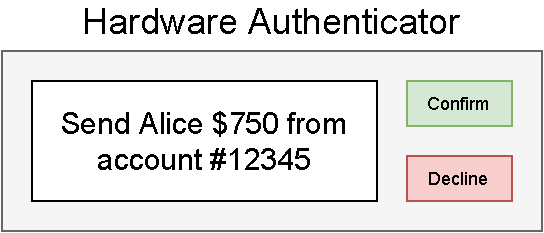
\includegraphics[width=10cm]{authenticator_drawio}
  \caption{User interface of hardware authenticator.}
  \label{Fig:HardwareAuthenticatorView}
\end{figure}

%% 
%% \iffalse
%% In the adversarial event that Alice were in fact malicious

%%  and the monetary transfer is actually intended for Bob

%% the user's web-browser were compromised and attempts to perform this unintended monetary transfer, 
%% \fi
%% 

This message contains enough information such that the user is fully informed of the operation they are about to perform. They can then make the educated judgment for whether to confirm the operation or not. In the adversarial event where a modified or unsolicited monetary transfer is attempted, the user should notice a discrepancy in the authentication message and decline the operation on the hardware authenticator. 

The goal of transaction authentication is to prevent the adversary from launching unsolicited operations on behalf of the user and causing fraudulence or damage. The operations that matter will require this additional authentication which the adversary cannot falsify as per the threat model --- the hardware device is assumed secure. This is a safe assumption because the hardware device is specialized to only perform this authentication process and nothing else. Ideally, it has a small attack surface that is vetted by security specialists. 

When the user authorizes this high-risk operation on their hardware authenticator, the message is cryptographically signed by the authenticator and sent back to the verifying end where it is checked. Only then, upon successful verification is the operation performed. 

Which operations should be protected is entirely at the discretion of the administrator of the web service. There is no clear-cut formula on what to protect, but candidate high-risk operations could include, but are not limited to, deleting one's account, transferring money, managing administrative permissions, publishing important software releases, etc. 


%% 
%% \iffalse

%% A security mechanism needs to protect against a stronger threat model in order to further harden a website's security. The threat model can be extended to where most of the transmission chain: the host computer, the operating system, web-browser, network and any other intermediate system may be compromised. And even under such a far-reaching threat model, the security mechanism must prevent unauthorized adversarial operation. What is assumed secure includes only the server code and hardware authenticator, as well as the entire registration event.

%% Traditional two-factor authentication may be simply extended as proposed by the WebAuthn specification \cite{TODO-WebAuthn} released by the World-Wide-Web Consortium (W3C) to work within this new and more restrictive threat model to defend against the class of vulnerabilities not covered by traditional two-factor authentication. This extension is called transaction authentication (txAuthn), and its goal is to enable "high-risk" operations to be individually authenticated by the user's hardware authenticator, despite the user being already logged in.

%% More specifically, when the user tries to issue some high-risk operation, they will be prompted with a message displayed on their paired hardware authenticator. The message is specific to the operation the user is trying to do, and should contain enough information needed for the user to verify that this is indeed the correct operation they want to perform. Upon acceptance by the user, the message is cryptographically signed by the hardware authenticator and sent back to the server where it gets verified, and only then, upon successful verification, is the operation performed.

%% A website, which assumes the more advanced threat model as described, would use transaction authentication to prevent any high-risk operations from being maliciously issued on behalf of the user. Such high-risk operations include, but are not limited to, deleting one's account, transferring money, managing administrative permissions, publishing important software releases, etc. 

%% For example, a bank website could require that monetary transfers exceeding \$500 must be transaction authenticated. In such a case, a possible authentication message that the user would have to confirm could resemble ``Send Alice \$750 from account \#12345''. This message contains enough information such that the user is fully informed as to what operation they are performing. Additionally, in the event that Alice is malicious and the transaction was actually intended for Bob, the user should notice this discrepancy in the authentication message and decline the operation on the hardware authenticator. 

%% \fi
%% 

%% 
%% \iffalse
%% The security benefits brought by transaction authentication to a web service would have a very tangible effect on the website's overall security. Client-side users of the application would have more faith that the website is operating correctly and not doing anything unauthorized at an adversary's request. Administrators of the website would rest more peacefully knowing that even if an adversary got access to their admin panel, they would not be able to do much damage as the critical operations require authentication from a physical hardware devices. And in general as a whole business, greater security would curb unnecessary losses due to hacker exploits and bolster greater trust in the general public's eye.
%% \fi
%% 

\section{Status Quo of Transaction Authentication}\label{Sec:StatusQuo}

%% 
%% \iffalse
%% Although transaction authentication is described in the WebAuthn protocol specification, no service or hardware authenticator has support for it. 
%% \fi
%% 

Although there are web services and hardware authenticators that support WebAuthn two-factor authentication, no service or authenticator supports the transaction authentication extension. Apart from transaction authentication not being integrated into real-world applications, there also has been no investigation into the implications of where it fits well, where it is inhibitory or unnecessary, what it takes to support transaction authentication in a web service and any software system designs that would help with integrating and configuring WebAuthn for an existing service.

%% 
%% \iffalse
%% In every case, there is what appears to be an almost standard practice for how WebAuthn gets used and integrated into a web service.
%% \fi
%% 

There are several publicly available codebases in the form of demo applets and libraries that work with WebAuthn transaction authentication~\cite{webauthn-online-examples} which illustrate how it can be used in a website. A website typically consists of a frontend and a backend. The frontend is the HTML/CSS/JavaScript that runs in the user's web-browser and is the origin of all of the user's requests when interacting with the website. The backend consists of the server code and database that execute the user's requests from the frontend. 

A web service using WebAuthn transaction authentication would have the frontend issue the WebAuthn requests and have the backend contain the WebAuthn library code to verify those requests and permit the operation if validation passes. Such approach to integrating WebAuthn has a number of practical downsides. 

%% 
%% \iffalse
%% Although this is a straightforward approach and is reasonable for a small applet web service, it begins to suffer when used on a larger codebase where the backend is complicated. 
%% \fi
%% 

Firstly, the backend architecture might not lend itself well to the control flow of the WebAuthn specification. In order to validate a WebAuthn request, multiple HTTP requests need to be sent back and forth between the frontend and backend. This may not be handled well by the backend if it was built under the assumption that there is only one HTTP request per operation.

Secondly, the integration of WebAuthn transaction authentication into a backend web service tends to be challenging for larger web services. The handler code for each operation is spread throughout the codebase, so it is difficult to keep track of what is secured and where in the code it is. Also, it requires a strong overall understanding of the web service code, which comes with its own set of challenges and slow development speed.

Lastly, in the extreme, albeit unlikely case, the backend may not even be accessible to the software developer if it is, for example, a closed-source API backend. In this case it is impossible to integrate WebAuthn into such a backend.

\section{Thesis Contributions}

There are three major contributions of this thesis:

\begin{enumerate}[nosep]

\item \sys{}: A firewall system design for integrating WebAuthn transaction authentication into a new or existing web service.

\item Three distinct case studies showcasing \sys{}. Each case study observes a class of web service and is used to test the limits of the usability of \sys{}.

\item A discussion on the beneficial use cases for transaction authentication, when it makes sense to be applied and when not.

\end{enumerate}

%% 
%% \iffalse
%% A second contribution is the use of the firewall in three distinct case studies.  The last contribution is a discussion on proper (and improper) usage of WebAuthn transaction authentication.
%% \fi
%% 

\subsection{WebAuthn Firewall}

Firstly, it must be emphasized that WebAuthn is simply a protocol specification. Implementation details are not bound to any one way, as long as they comply with the protocol's details. However, the code demos of WebAuthn unanimously integrate it into their codebases in the same intrusive manner. They import a WebAuthn library~\cite{webauthn-library} directly into the codebase and perform the necessary checks and validation in the backend.

\begin{figure}[h]
  \centering
  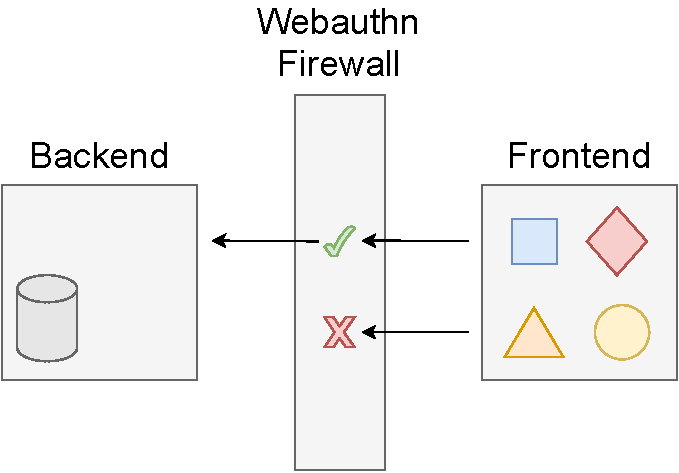
\includegraphics[width=12cm]{firewall_drawio}
  \caption{Basic depiction of the WebAuthn firewall functionality.}
  \label{Fig:BasicFirewallDepiction}
\end{figure}

This thesis proposes an alternative method for integrating WebAuthn by incorporating \sys{}, a Web Application Firewall (WAF). This firewall monitors and filters HTTP traffic sent from the website webpage to the backend. Any requests that the firewall deems as needing WebAuthn transaction authentication are stopped and processed by it. The firewall validates the request according to the WebAuthn transaction authentication specification. Figure~\ref{Fig:BasicFirewallDepiction} depicts how if the validation succeeds, then the firewall lets the request pass on through to the backend. If not, then the request is blocked. As far as the backend is concerned, it is unaware that \sys{} exists between it and the website webpage. 

With the WebAuthn firewall approach, the backend has to be minimally, if at all, modified to support WebAuthn transaction authentication. Although the frontend still needs to be modified to produce the WebAuthn transaction authentication requests as it is the origin of all of the user's operations, the firewall approach lends itself better to integrating WebAuthn into a new or existing web service. It is less intrusive than the traditional library-based approach and consolidates all of the WebAuthn related code in one place. As a result, it is less error-prone and easier to configure. 

%% 
%% \iffalse
%% . Needless to say, such a system design 
%% \fi
%% 

%% TODO: Is mentioning that the firewall is its own application, independent of the frontend or backend, worthwhile?

%% 
%% \iffalse
%% Additionally, the WebAuthn firewall is independent of the frontend and backend. 
%% \fi
%% 

The design of \sys{} presented in this thesis goes beyond simply providing a description and base functionality. It supplies the software engineer with useful defaults and a domain specific language (DSL) to configure \sys{}. Namely with a short configuration, the engineer can adapt \sys{} to parse and understand whatever input request format the web service uses. Requests map to operations in a web service depending on which HTTP route they are sent to. With only a few lines of code per route in the \sys{} configuration, the engineer can specify that the route be checked with transaction authentication and what the authentication message should be in order to pass as valid for that operation. 

%% 
%% \iffalse
%% The firewall handles the back-and-forth HTTP requests required for WebAuthn authentication. 

%% So it is much easier for the software engineer to organize and control what operations need transaction authentication and how exactly they get secured. 
%% \fi
%% 

%% 
%% \iffalse
%% % TODO: Are there demos for txAuthn or just WebAuthn. I think the latter only
%% Despite no major applications of WebAuthn, there are several publicly available codebases in the form of demo applets and libraries that work with WebAuthn \cite{TODO-WebAuthn-codebases-from-WebAuthn-website}. In every case, there is what appears to be an almost standard practice for how WebAuthn gets used and integrated into a service. A website typically consists of a frontend and a backend. The frontend is the web code that runs in the user's web-browser and is the origin of all of the user's requests when interacting with the website. The backend consists of the server code and database store that actually operates the website. Traditionally a web service using WebAuthn would have the frontend issue the WebAuthn requests and have the backend contain the code to verify those requests and permit the operation if everything passes. The principal contribution of this thesis demonstrates that there are alternative methods to using and integrating WebAuthn.
%% \fi
%% 

\subsection{Case Studies}

\begin{figure}[h]
  \centering
  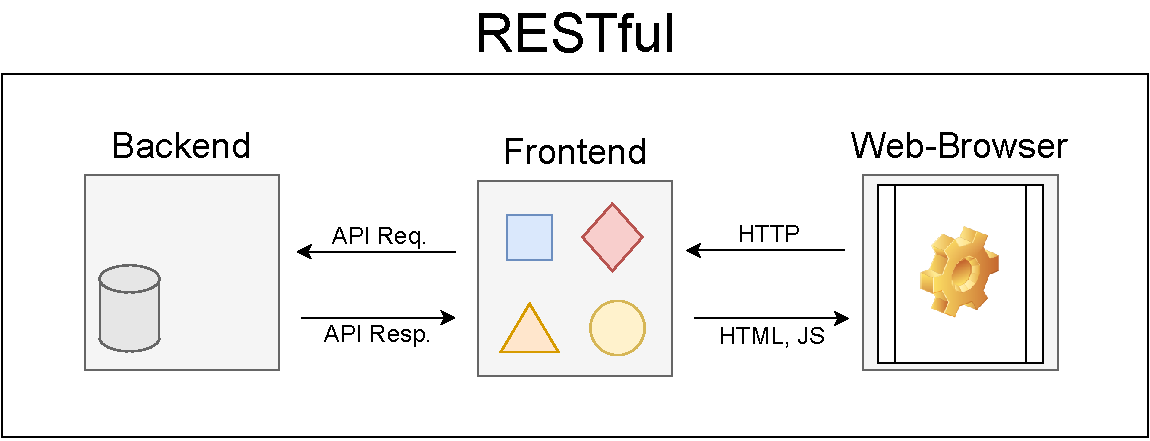
\includegraphics[width=10cm]{RESTful_drawio}
  \caption{The architecture design of a RESTful web application.}
  \label{Fig:CaseStudiesRESTful}
\end{figure}

\begin{figure}[h]
  \centering
  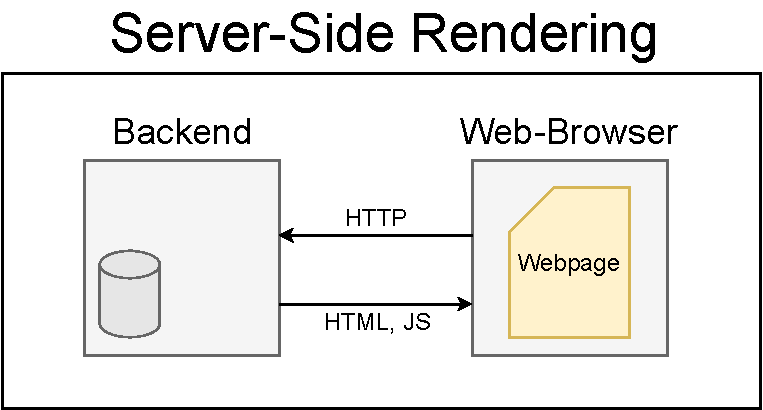
\includegraphics[width=9cm]{ServerSide_drawio}
  \caption{The architecture design of a server-side rendering web application.}
  \label{Fig:CaseStudiesServerSide}
\end{figure}

Three separate case studies demonstrate how \sys{} secures different architectures of web applications with WebAuthn transaction authentication. The web applications studied cover the RESTful design paradigm and the more traditional server-side rendering paradigm. The two RESTful applications studied are Conduit~\cite{conduit}, a simple blogging website, and Calypso~\cite{calypso}, a frontend admin panel for WordPress. As illustrated in Figure~\ref{Fig:CaseStudiesRESTful}, the RESTful paradigm is where the frontend runs in the web-browser separately from the web server backend program. The frontend performs the rendering visible to the user, and whenever it needs to fetch information or has to perform some server operation, it communicates via a pre-established API to the web server, which executes those requests. 

The server-side rendering application studied is Gogs~\cite{gogs}, a self-hosted Git service much like GitHub~\cite{github}. Figure~\ref{Fig:CaseStudiesServerSide} depicts the server-side rendering paradigm, where every operation the user performs on the webpage is sent over to the server as an HTTP request. In response, the server returns a whole new webpage, complete with all of the HTML and JavaScript code to be displayed on the user's web-browser.

%% 
%% \iffalse
%% . In return, everything that the user sees gets rendered on the server and is sent back as HTML code to be displayed directly by the user's web-browser.
%% \fi
%% 

These case studies stress test the flexibility and configurability of \sys{}. They are critical in establishing what parameters and configurable knobs \sys{} should provide. They are also used to evaluate how tangible the improvements are for using \sys{} in a web service rather than integrating WebAuthn transaction authentication intrusively. 

%% 
%% \iffalse
%% Lines of code, complexity, configurability, and integration difficulty are all evaluation criteria which support the use of the WebAuthn firewall over the traditional method.
%% \fi
%% 

\subsection{Other WebAuthn Possibilities}

In this thesis, Chapter~\ref{Chap:DiscussionAndFutureWork} gives insights into best practices relating to utilizing WebAuthn transaction authentication to secure various classes of problems. Researching transaction authentication reveals clear use cases where it lends itself well to secure, some use cases which are possible to secure, but not optimal, and lastly some use cases which cannot be protected at all by transaction authentication. 

%% 
%% \iffalse
%% There is future work that builds on from some of the insights provided by this research. web service routes can be analyzed to verify there is no way to subvert any protected routes. Also transaction authentication can be used to lessen how much code in the transmission chain must be trusted, to provide an even stricter threat model than the one assumed for the WebAuthn firewall. 
%% \fi
%% 

%% 
%% \iffalse
%% \subsection{WebAuthn Status Quo}

%% Firstly, it must be emphasized that WebAuthn is simply a protocol specification. Implementation details are not bound to any one way, as long as they comply with the protocol's details. However, the code demos of webauthn unanimously integrate it into their applet services in the same intrusive manner. They import a webauthn library in one of the many supported languages~\cite{TODO-webauthn-libraries} that performs the various validity and authentication checks along the webauthn specification. Then directly in the applications codebase, they invoke the library where it webauthn security is needed. This is a very straightforward coding practice and is very reasonable for a small applet web service. However, the same approach begins to suffer when used on a larger codebase when the backend is complicated and its architecture might not even lend itself well to the control flow of the webauthn specification. In order to validate a webauthn request, multiple HTTP requests need to be sent back and forth between the frontend and backend. This may not be handled well by the backend if it was built under the assumption that one HTTP request per operation. In other cases, the backend is fully inaccessible because it is part of a closed-source software project. 

%% \subsection{Overview of Contributions}

%% An alternative method for integrating webauthn is as a Web Application Firewall (WAF). This firewall monitors and filters HTTP traffic sent from the frontend to the backend. Any requests that the firewall deems as needing further webauthn transaction authentication get stopped. The firewall handles the back-and-forth HTTP requests required for webauthn authentication. And if all succeeds, it lets the request pass on through to the backend. As far as the backend is concerned, it is virtually unaware that a firewall exists between it and the frontend performing the webauthn validation. Under such webauthn firewall approach, the backend has to be minimally, if at all, modified to support webauthn transaction authentication. The frontend still needs to be modified to produce the webauthn transaction authentication requests as it is the origin of all of the user's operations. Needless to say, such a system design lends itself much better for integrating webauthn into a new or existing web service. It is much less intrusive than the traditional library-based method. As a result, it is much less error-prone and easier to configure. Additionally, the webauthn firewall is independent of the frontend and backend. So it is much easier for the software engineer to organize and control what operations need transaction authentication and how exactly they get secured. 

%% The webauthn firewall presented in this thesis goes beyond simply providing base functionality. It supplies the software engineer with useful defaults and a powerful domain specific language (DSL) to configure the firewall. Namely with a short configuration, the engineer can adapt the firewall to parse and understand whatever input request format the web service uses. Additionally, with only a few lines of code per HTTP route, they can also specify that the route gets checked with transaction authentication and what the authentication message should be in order to pass as valid for that operation. 

%% Furthermore, case studies demonstrate how the webauthn firewall secures three different architectures of web applications with webauthn transaction authentication. The web applications studied cover the RESTful design paradigm and the more traditional server-side rendering paradigm. The RESTful paradigm is where the webpage frontend and web-server backend are two separate programs. The frontend performs the rendering visible to the user, and whenever it needs to fetch information or has to perform some server operation, it communicates via a standardized API to the web-server which executes those requests. The server-side rendering paradigm is where every operation the user performs on the webpage gets requested to the server directly. In return, everything that the user sees gets rendered on the server and is sent back as HTML code to be displayed directly by the user's web-browser.

%% These case studies stress test the flexibility and configurability of the webauthn firewall. They were critical in establishing what parameters and configurable knobs the firewall should provide. They are also used to evaluate how tangible the improvements are for using the firewall in a service rather than more traditionally integrating webauthn transaction authentication intrusively. Lines of code, complexity, configurability, and integration difficulty are all evaluation criteria which support the use of the webauthn firewall over the traditional method.

%% Beyond describing the webauthn firewall, the thesis will also give insights into best practices relating to utilizing webauthn transaction authentication to secure various classes of problems. Researching transaction authentication revealed clear use cases where it lends itself well to secure, some use cases which are doable to secure, but not optimal, and lastly some use cases which are not protected at all be transaction authentication. There is future work that builds on from some of the insights provided by this research. web service routes can be analyzed to verify there is no way to subvert any protected routes. Also transaction authentication can be used to lessen how much code in the transmission chain must be trusted, to provide an even stricter threat model than the one assumed for the webauthn firewall. 
%% \fi
%% 

%% 
%% \iffalse
%% in order a protected operation to be processed by the web-server, it must be 

%% but it is not void of vulnerabilities

%% with only a few lines of code per HTTP route, the engineer can adapt the firewall to parse and understand whatever input request format the web service uses. 

%% specify whether the route gets checked with transaction authentication and what the authentication message should be to pass as valid for that operation. 

%% Each  how well it can support a variety of different web applications, each with different 
%% \fi
%% 

\subsection{Source Code}

The source code of \sys{} and case studies is publicly available at \url{https://github.com/JSmith-BitFlipper/Guarda-firewall} under the MIT License.

%% 
%% \iffalse
%% Cheers! 
%% \fi
%% 

\section{Thesis Outline}

The thesis contains the following chapters. Chapter~\ref{Chap:RelatedWork} discusses the related work and background pertinent to this research. Chapter~\ref{Chap:WebauthnTransactionAuthentication} describes the WebAuthn transaction authentication protocol in detail. Chapter~\ref{Chap:WebauthnFirewallDesign} outlines the design of \sys{}, the WebAuthn firewall. Chapter~\ref{Chap:WebauthnFirewallImplementation} discusses the implementation details of the novel components of \sys{}. Chapter~\ref{Chap:CaseStudies} explains the case studies of \sys{}. Chapter~\ref{Chap:Evaluation} contains the experiments and evaluation metrics for \sys{}. Chapter~\ref{Chap:DiscussionAndFutureWork} opens a discussion of supplemental notes uncovered over the course of this research. Finally, Chapter~\ref{Chap:Conclusion} concludes this thesis.

%% This is an example first chapter.  You should put chapter/appendix that you
%% write into a separate file, and add a line \include{yourfilename} to
%% main.tex, where `yourfilename.tex' is the name of the chapter/appendix file.
%% You can process specific files by typing their names in at the 
%% \files=
%% prompt when you run the file main.tex through LaTeX.
\chapter{Related Work}\label{Chap:RelatedWork}

This chapter presents the background and related work that precedes this research. These concepts lay out the foundation on which the rest of this research is conducted.

% TODO: Maybe explain what external observation and internal observation are
\section{Hardware Authenticators for \newline Two-Factor Authentication}\label{Sec:HardwareAuthenticators_2FA}

The state of the art for using hardware devices for website authentication is two-factor authentication. These devices such as the YubiKey \cite{yubico-products} resemble a small USB key which stores a private key on device. Websites that support two-factor authentication simply request the secondary mode of authentication during login. Two-factor authentication solves the security problems for login quite well \cite{questRemovePasswords}. Depending on the implementation of the specific hardware device, most provide strong resilience to targeted impersonation, physical observation, internal observation, leakage of data secrets and relying on a trusted third-party. However, as explained previously, these benefits do not pertain beyond the login point of a website and assume a lenient threat model. The adversary with control over the web-browser could simply wait for the user to faithfully log in and then launch their planned attack. 

%% 
%% \iffalse
%% , in addition to supplying a password. 
%% \fi
%% 

A number of specifications standardize two-factor authentication so that the same hardware authenticator device may be used across platforms and web services. A popular standard is Universal 2nd Factor (U2F) \cite{fido-u2f} developed by Google and Yubico, now hosted by the open-authentication industry consortium FIDO (``Fast IDentity Online'') Alliance. It is succeeded by FIDO2 \cite{fido2}, which merges WebAuthn and its extensions, including transaction authentication, into one common standard.

\section{Current Uses of Transaction Authentication}\label{Sec:CurrentUses_txAuthn}

Although transaction authentication by the WebAuthn standard is not yet commonly used, cryptocurrency hardware wallets universally support transaction authentication. The two most popular manufacturers, Ledger \cite{ledger} and Trezor \cite{trezor}, sell hardware wallets which hold the private keys and have displays. In order to send any cryptocurrency from the device, the device displays a message detailing the transaction, which the user would need to authorize on the physical device. Otherwise, the device will not sign the transaction which is required for it to proceed and be sent over the network.

In a similar but diminished vain, some banks such as Bank of America reuse two-factor authentication for sensitive or high-value monetary transactions \cite{BoA-2FA}. In order to complete the sensitive transaction, the user must redo two-factor authentication like during login. This is unlike transaction authentication in that no hardware device specific to transaction authentication is involved, and the user does not see a confirmation of the exact transaction to take place before confirming. But the process of requesting supplemental two-factor authentication on sensitive transactions aims to defend against a similar threat model as transaction authentication.

\section{Hardware Authenticators for \newline Transaction Authentication}

Hardware authenticator devices normally do not support general-purpose transaction authentication. Hardware authenticators for two-factor authentication such as the YubiKey discussed in Section~\ref{Sec:HardwareAuthenticators_2FA} do not have any display. Therefore, they are unable to perform the core function of transaction authentication, displaying a message to the user and signing it upon their confirmation. The cryptocurrency hardware wallets discussed in Section~\ref{Sec:CurrentUses_txAuthn} provide transaction authentication, but only for a limited subset of functionality relating to crypto transactions.  

%% 
\iffalse
, but none support the transaction authentication extension.

are dedicated hardware devices required by the threat model. Also, these authenticators only support regular WebAuthn two-factor authentication, not the transaction authentication extension. 
\fi
%% 

WebAuthn transaction authentication is not supported by any hardware authenticators. A few hardware authenticators and software emulated authenticators support WebAuthn, but only the regular two-factor authentication. The software emulated authenticators are intended for development and research purposes. Google has a Chrome extension that poses as a virtual hardware authenticator; it performs all of the signing in-browser \cite{virtual-authenticators-tab}. Krypton is a small company dedicated to making cryptographic authentication easy \cite{krypton}. They provide a browser plugin and phone app, which pair with one another. The plugin interfaces with the web-browser and the phone performs the cryptographic signing. 

This research must modify one of the software emulated authenticators to support transaction authentication. It uses a modified Krypton browser plugin to display the authentication message and await user consent before performing the signing also in-browser. Figure~\ref{Fig:KryptonAuthenticator} portrays the user interface of the plugin as it awaits consent before returning a signed transaction authentication object. This design deviates from the original Krypton design since it eliminates the phone app from the signing process. The security properties of the authenticator device itself is not a focus for this research. It is assumed always secure, so for prototyping and experimentation, this software modified authenticator is sufficient.

\begin{figure}[h]
  \centering
  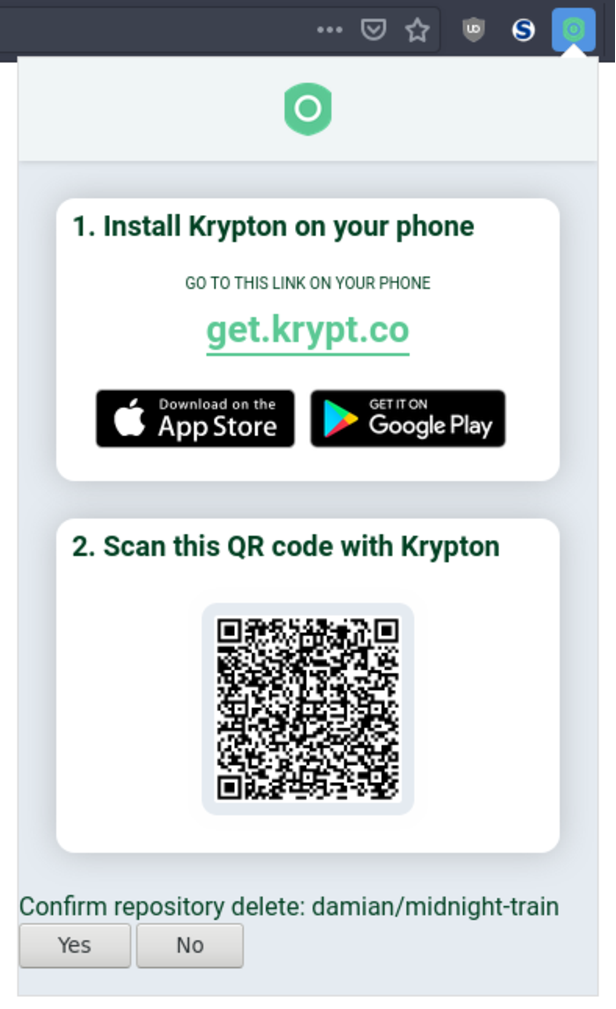
\includegraphics[width=10cm]{krypton_txauthn}
  \caption{User interface of Krypton authenticator in this thesis. It is awaiting user consent before authorizing the deletion of a repository ``damian/midnight-train''.}
  \label{Fig:KryptonAuthenticator}
\end{figure}

%% 
%% \iffalse
%% For ease of development, this research modified the Krypton browser plugin to display the authentication message and await user consent before performing the signing in-browser. It completely

%% Since the design of the hardware authenticator is not a focus for this research, it is simpler to avoid interfacing with the phone at all. 
%% \fi
%% 

\section{Web Application Firewalls}

A Web Application Firewall is a firewall that filters web traffic going to a web service \cite{web-application-firewall}. Most web application firewalls try to block malicious internet traffic from ever reaching the web server. Common attacks defended against by web application firewalls include SQL injection, cross-site scripting and DDoS attacks. Typically, the firewall inspects incoming GET and POST request HTTP/HTTPS traffic and applies pre-configured rules to identify and filter out the undesired traffic. This thesis describes how to make a web application firewall supporting WebAuthn transaction authentication.


%% 
%% \iffalse

%% This research builds on top of the description of transaction authentication as outlined by the first version of the webauthn specification \cite{webauthn}. The webauthn specification is a comprehensive document, standardizing a protocol for two-factor authentication with configurable extensions. The protocol covers in detail how traditional two-factor authentication should be performed under webauthn as well as details how to extend it to perform transaction authentication. Transaction authentication is similar to a regular two-factor authentication event, just with some additional user involvement; the user must confirm a given transaction on a dedicated hardware device for the authentication to proceed. 

%% The purpose of transaction authentication in the eyes of the webauthn specification authors is to provide integrity to high risk operations on a website. In fact, further papers including \cite{EuroFIDO} detail use-cases of webauthn transaction authentication such as authorizing large value monetary transactions, consenting to data being shared with a third-party and authorizing a trusted service to sign a digital contract. All of these operations are very important and requesting individual authentication for each may be warranted. 

%% It appears that the state of the art for known security benefits through transaction authentication ends there. There is no research detailing how webauthn transaction authentication should be integrated into a service, what are good design choices in doing so or what the engineer should keep in mind in order to avoid accidental security holes.

%% \fi
%% 

%% This is an example first chapter.  You should put chapter/appendix that you
%% write into a separate file, and add a line \include{yourfilename} to
%% main.tex, where `yourfilename.tex' is the name of the chapter/appendix file.
%% You can process specific files by typing their names in at the 
%% \files=
%% prompt when you run the file main.tex through LaTeX.
\chapter{Webauthn Transaction Authentication}\label{Chap:WebauthnTransactionAuthentication}

Webauthn transaction authentication is a protocol specification for authenticating high-risk user operations, even after login. The specification describes a sequence of steps that must be followed in order to authenticate properly. These steps can be split into four stages, registration, the setup, the cryptographic attestation and then the verification. 

\begin{enumerate}[nosep]
\item Registration: Makes a record of the user and their cryptographic credential into a database store later accessible to the verification code and is performed only once per user.

\item Setup: Initiated by the user's web-browser and involves a priming exchange between it and the webauthn verification end.

\item Cryptographic Attestation: Occurs on the hardware authenticator device after the user confirms the operation. The threat model assumes that this attestation is always secure.

\item Verification: Validates whether to authorize the high-risk user operation or not. Checks if the requested operation matches its authentication message and that the cryptographic signature on it is valid. This stage also is assumed secure under the threat model.

\end{enumerate}

This outline for transaction authentication uses the webauthn firewall as the verification end. It contains the database of user public key credentials and performs the validation to authorize high-risk operations or not. As webauthn is a protocol specification, nothing dictates this design choice. However, for continuity with the thesis work, the protocol is best explained with the firewall.

%% 
%% \iffalse
%% between the user and hardware authenticator device. 

%% Lastly, the verification stage 
%% Occurs within the firewall, and it 
%% \fi
%% 

\subsection{Webauthn Registration}

\begin{center}
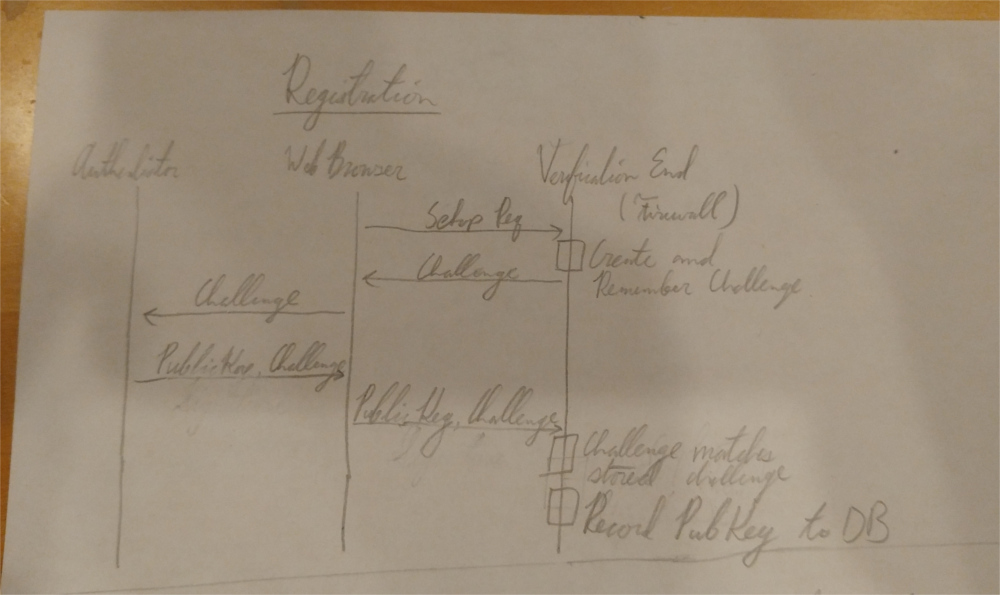
\includegraphics[width=12cm]{registration_flow}
\end{center}

During the registration event, the user's hardware device sends its public key credential to the firewall. This process is completely secure in the threat model, with no adversary to intercept or tamper with any of the communication. Therefore, whatever credential the firewall receives during registration is assumed to be genuine and the user's. The firewall later on uses this credential during the verification stage to ensure transaction authentication integrity. The registration process begins with a setup of its own, where the web-browser requests a few parameters from the firewall, most notably a random challenge nonce.

%% 
%% \iffalse
%% \begin{lstlisting}
%% type PublicKeyCredentialCreationOptions struct {
%% 	Challenge              Challenge                
%% 	RelyingParty           RelyingPartyEntity       
%% 	User                   UserEntity               
%% 	Parameters             []CredentialParameter
%% 	AuthenticatorSelection AuthenticatorSelection
%% 	Timeout                int                      
%% 	Attestation            ConveyancePreference
%% }
%% \end{lstlisting}
%% \fi
%% 

The firewall remembers the challenge it sent as a part of the session data associated with the registration setup request. The challenge nonce prevents replay attacks \cite{TODO-replay-attack}. There are a few other parameters, but they are mainly for the hardware device to know what type of credential the firewall is expecting to receive. The hardware device sends over its public key credential for the firewall to save, with the challenge signed by that credential. The firewall receives an HTTP POST request containing this public key credential. The POST request also contains identifying information of the current user. The firewall verifies that the challenge is matches, and upon success, stores the credential and associated user ID into a database row.

\subsection{Transaction Authentication Setup}\label{Sec:TransactionAuthenticationSetup}

\begin{center}
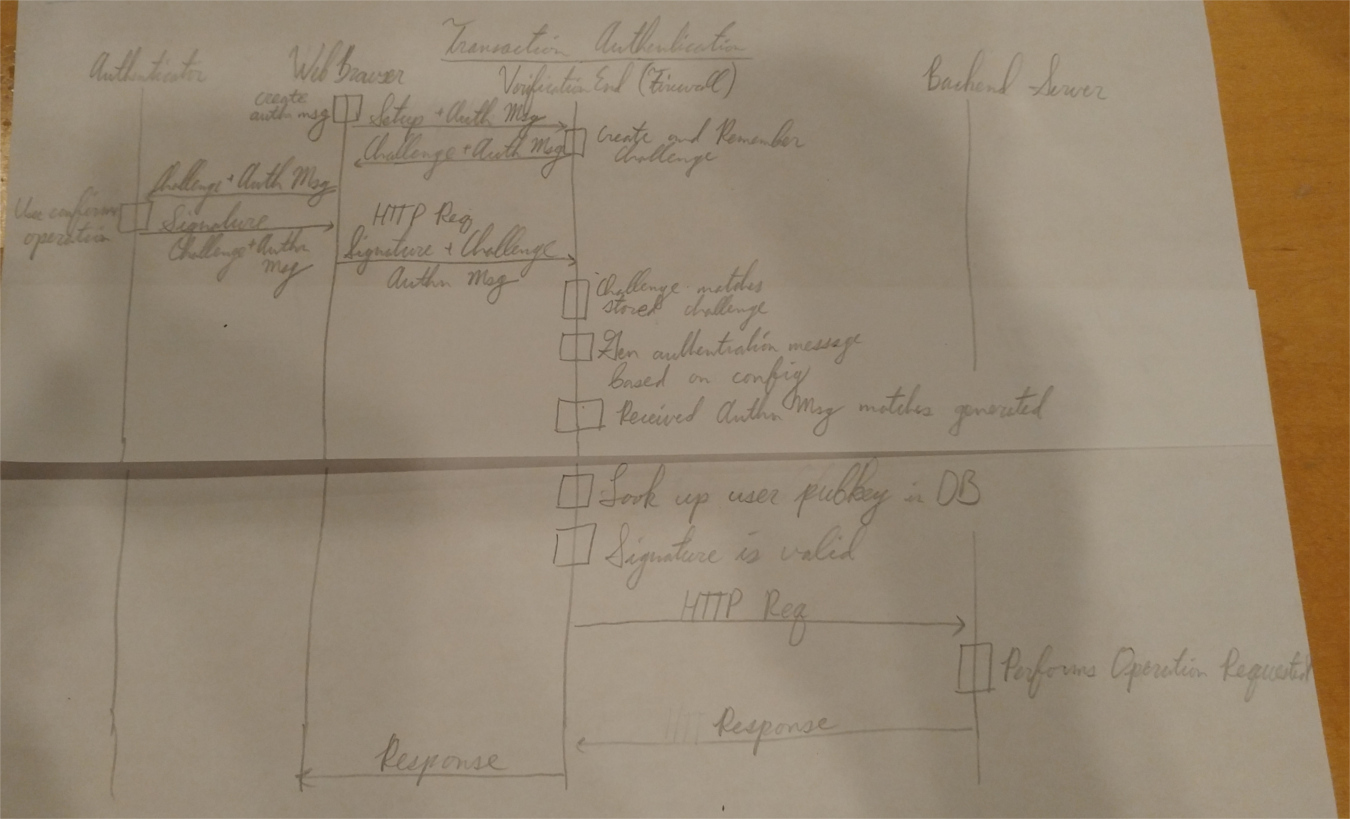
\includegraphics[width=15cm]{txauthn_flow}
\end{center}

% TODO: Talk about server-side rendering preloading

The setup for a transaction authenticate event generally originates from the frontend. There are several designs to setup a webauthn transaction event, but the setup content itself is all the same. More commonly, setup may occur lazily where the frontend waits for the user to initiate an operation protected by transaction authentication before initiating the setup. Or it may occur eagerly where the frontend preemptively initiates the setup, without knowing whether the user will even perform any secured operation on the web-page. Nonetheless, the setup is a POST request to the firewall. The payload for the setup POST request is an authentication message that will eventually be displayed to the user on their hardware device. The message is constructed from any user input and any additional information contained in the HTML of the webpage, but in all three case studies of this thesis, that was always enough. In response, the frontend receives a few parameters:

%% 
%% \iffalse
%% \begin{lstlisting}
%% type PublicKeyCredentialRequestOptions struct {
%% 	Challenge          Challenge                   
%% 	Timeout            int                         
%% 	RelyingPartyID     string                      
%% 	AllowedCredentials []CredentialDescriptor      
%% 	UserVerification   UserVerificationRequirement 
%% 	Extensions         AuthenticationExtensions    
%% }
%% \end{lstlisting}
%% \fi
%% 

Most importantly, a random \lstinline{challenge} nonce is returned. The firewall remembers it locally in the session data associated with the request. When the firewall processes the protected request, it will verify that the challenge included in the returned authentication data matches the one previously sent and remembered in the session. An adversary cannot intercept and replay old protected requests since it is exceedingly unlikely that future challenges from the firewall will exactly match the challenge in the intercepted request. 

An \lstinline{extensions} field is also returned, following the webauthn protocol. The firewall took the authentication message sent to it and transformed it into a form which any webauthn-compatible hardware authenticator should handle as a transaction authentication operation.

%% 
%% \iffalse
%% There are other fields returned as a part of the setup, but they are mostly for plumbing. They delineate how the hardware device should respond when authenticating the webauthn transaction.
%% \fi
%% 

%% 
%% \iffalse
%% The other fields are mostly for plumbing. The \lstinline{Timeout} requires an authentication response with that amount of time. The \lstinline{RelyingPartyID} identifies the backend. The \lstinline{AllowedCredentials} identifies with which cryptographic key the user can sign the response. The \lstinline{UserVerification} tells the hardware authenticator that the user must physically confirm ``yes'' or deny ``no'' a request and is usually set to \lstinline{true}. The \lstinline{Extensions} includes a signal that transaction authentication is to be performed with the authentication message sent to the firewall.
%% \fi
%% 

\subsection{Cryptographic Attestation}\label{Sec:CryptographicAttestation}

The request options from the firewall go through the frontend and are passed on to the hardware authenticator device. The threat model assumes that only the firewall, backend and hardware authenticator are secure. At any point, the frontend or web-browser could modify these options, but any tampering will be detected later on and denied authorization. The hardware device parses the request options, extracts from the \lstinline{extensions} field the authentication message and presents that to the user. The authentication message is in the form of a confirmation for some requested operation and is answered either by ``yes'' or ``no''. If the user attests ``yes'', the hardware device cryptographically signs a data object which is returned as an additional field within the HTTP request to the firewall for verification.

The response of the hardware authenticator includes a \lstinline{clientDataJSON} object containing the authentication message displayed to the user a well as the \lstinline{Challenge} from the setup stage. A cryptographic signature of the \lstinline{clientDataJSON} is also included. Specifically, Elliptic Curve Digital Signature Algorithm (ECDSA) paired with the SHA-256 hash function is the signing function. There are other fields, as well, for plumbing to help the firewall know what parameters to use to validate this response.

%% 
%% \iffalse
%% % TODO: Make this typescript highlighting
%% \begin{lstlisting}
%% const credential: PublicKeyCredential = {
%%     id: string, // base64 encoded
%%     rawId: []bytes,
%%     response: {
%%         attestationObject: []bytes,
%%         clientDataJSON: {
%%             challenge: string, // base64 encoded
%%             clientExtensions: []bytes,
%%             hashAlgorithm: string,
%%             origin: string,
%%         },
%%     },
%%     type: 'public-key',
%% };
%% \end{lstlisting}

%% The \lstinline{clientDataJSON} contains the \lstinline{clientExtensions} which is the data displayed to the user as well as the \lstinline{challenge} from the setup stage. The cryptographic signature of the \lstinline{clientDataJSON} is included in the \lstinline{attestationObject} and uses the Elliptic Curve Digital Signature Algorithm (ECDSA) paired with the SHA-256 hash function. The other fields are for plumbing and help the firewall know what parameters to use to validate this authentication data object.
%% \fi
%% 

\subsection{Webauthn Firewall Verification}\label{Sec:WebauthnFirewallVerification}

The webauthn firewall receives an HTTP request on a protected route with all of its usual parameters plus the authentication data object. The firewall must verify the integrity of this object as well that it corresponds with the intent of the HTTP request. In other words, it must detect whether any code not in the trusted computing base, such as the frontend, tampered with the authentication data. Also, it must make sure that the operation the user attested to on their hardware device that resulted in this authentication data object is in fact the operation to be performed if the protected HTTP request were to be permitted through. The three main steps of this verification are checking the challenge, the authentication message and the authentication data signature.

Checking the challenge is a simple comparison between the challenge received \lstinline{challenge} and the \lstinline{storedChallenge} in the firewall's session data. This protects against replay attacks.

%% 
%% \iffalse
%% \begin{lstlisting}
%% // Verify the challenge
%% Challenge := c.ClientDataJSON.Challenge
%% if strings.Compare(storedChallenge, Challenge) != 0 {
%% 	err := ErrVerification.WithDetails("Error validating challenge")
%% 	return err
%% }
%% \end{lstlisting}
%% \fi
%% 

Checking the authentication message is slightly more involved. The firewall is configured per route how to generate an expected authentication message based on the HTTP request parameters. This generated authentication message must unambiguously encapsulate the entire intent of the request. Details are further discussed in Section~\ref{Sec:AuthenticationMessage}. Then it is a simple comparison between the received \lstinline{clientMessage} and the \lstinline{generatedMessage}. This makes sure the user authenticated a message that faithfully represents the intent of the HTTP request.

%% 
%% \iffalse
%% \begin{lstlisting}
%% // Verify the authentication message
%% clientMessage := c.ClientDataJSON.Extensions["txAuthnSimple"]
%% if strings.Compare(generatedMessage, clientMessage) != 0 {
%% 	err := ErrVerification.WithDetails(
%%               "Error validating authentication message")
%% 	return err
%% }
%% \end{lstlisting}
%% \fi
%% 

Lastly, checking the authenticating data signature involves invoking cryptography library utilities. This validates the integrity of the entire authentication object to prove that it was not tampered with. The \lstinline{clientDataJSON} was signed by the hardware authenticator. The firewall has the public key of the hardware authenticator, so it can see if the \lstinline{clientDataJSON} indeed corresponds to the signature attributed to it.

%% 
%% \iffalse
%% \begin{lstlisting}
%% // Verify the signature

%% // The data signed by the hardware authenticator
%% clientDataHash := sha256.Sum256(c.ClientDataJSON)
%% sigData := append(p.Raw.AssertionResponse.AuthenticatorData, 
%%                   clientDataHash[:]...)

%% // The user's public key stored in the firewall
%% key, err := webauthncose.ParsePublicKey(credentialBytes)
%% valid, err := webauthncose.VerifySignature(
%%                  key, sigData, p.Response.Signature)
%% if !valid {
%% 	return err
%% }
%% \end{lstlisting}

%% Setup can occur eagerly where the web-browser immediately performs the setup without the user initiating any operation protected by transaction authentication.

%% If not, it will deny the request from continuing through.

%% The frontend only has access to the information it displays in the HTML to the user, 

%% The data displayed to the user along with its respective signature is included in the \lstinline{response} field. The hardware device signs
%% \fi
%% 

%% This is an example first chapter.  You should put chapter/appendix that you
%% write into a separate file, and add a line \include{yourfilename} to
%% main.tex, where `yourfilename.tex' is the name of the chapter/appendix file.
%% You can process specific files by typing their names in at the 
%% \files=
%% prompt when you run the file main.tex through LaTeX.
\chapter{Webauthn Firewall Design}

The webauthn firewall acts as a Web Application Firewall (WAF). It is situated directly between the frontend and backend, processing all user requests sent between the two. Each requests gets parsed by the firewall, and understood whether it is a request that needs webauthn transaction authentication or not. If not, the request is simply proxied through to the backend without any extra work. However, if it needs transaction authentication, the firewall as a gatekeeper for that request. The firewall performs a verification procedure on the request and only upon success does the request pass through the firewall to the backend. If it fails, the firewall returns an error back to the frontend. This design strategy for integrating webauthn transaction authentication into a service is very powerful because it is web service agnostic. The backend is completely unaware that the requests it receives are webauthn authenticated. Of course, since the frontend has to interface with the user's hardware authenticator device, it must be aware of webauthn, but only to a minor extent. 

\subsection{Proxying Requests}

In multiple case studies, the firewall was used to integrate webauthn transaction authentication into two different paradigms of web service designs, RESTful and server-side rendered websites. For each, the notion of the firewall being situated between the frontend and backend is slightly different, but the function and role of the webauthn firewall is the same, filtering, verifying and proxying requests. For a RESTful web application, the placement of the firewall is more intuitive. In a RESTful design, frontend and backend are separate programs running on their own IP addresses and ports. The user's web-browser interacts with the frontend through its IP address. And whenever the frontend needs to interact with the backend, it launches HTTP requests to the IP address of the backend. In a RESTful web service design, the webauthn firewall naturally sits in between the two. The firewall runs on its own IP address and port, and the frontend is reconfigured to use it as its backend address destination. So when the frontend needs to issue a backend request, it sends it rather to firewall rather than the backend. From there, the firewall performs its role and, as necessary, proxies onward to the actual backend. Responses from the backend are returned to the firewall which automatically get forwarded on to the frontend. In a server-side rendering web application, the firewall additionally performs the role of the frontend described in the RESTful use case. That is, the user's web-browser interacts with the IP address of the firewall directly. All HTTP requests originate from the user's web-browser and are directed to whatever the address is of the frontend. In a server-side rendering web application, the whole service, the frontend and backend, is served out of the same address. With the webauthn firewall, requests get sent to the firewall which again does its role and, if necessary, relays onward to the server-side rendering web-application. In this case, the webauthn firewall is situated between the web-browser and backend. But nonetheless, it is the same principle as with the RESTful web application use case. An origin, in this case the web-browser, issues requests destined for a backend, but they get intercepted by the firewall, before they continue on if everything succeeds.

\subsection{Webauthn Verification}

% TODO: Make option in firewall to either pass through or block non-specified requests. Modify this paragraph
% TODO: Explain basic webauthn txAuthn ecosystem

As the webauthn firewall filters requests sent to it, some requests will be held back to be webauthn transaction authenticated first. Which requests get held back and how they get verified is configured in the firewall by the software engineer. In order to specify which HTTP route to filter out and transaction authenticated, the engineer simply includes the route in the firewall's configuration. All other routes not specified in the configuration are simply passed on through to the backend without any checks.

\subsubsection{Authentication Message}

Of the requests that need to be checked, the engineer must specify how they get verified. In essence, verifying an incoming HTTP request with transaction authentication involves the firewall generating an authentication message from the parameters of the request. Then the verification passes only if the generated message is exactly identical to the message signed by the hardware authenticator also included in the request and the associated signature is valid. The message generated by the firewall represents the root of truth and should encapsulate the entire intent of the request in order to have good security guarantees. All of the parameters in the requests that are considered security sensitive must appear unambiguously in the authentication message in a human readable format. Unambiguity refers to how no two different requests can share the same authentication message. Human readability is critical since the user is the one authenticating the message and sometimes the parameters in the request may be not human intelligible such as object IDs, etc.

\subsubsection{Context Retrieval}

% TODO gets context

Where the HTTP request contains not human friendly identifiers that need to be understood by the user, those identifiers must be translated to their human readable counterparts. For example, an ID may identify some object in a web service. The firewall must generate...

\iffalse
is reconfigured to issue backend requests to the IP address

Upon opening the web page, requests are issued from the web-browser

has two options to specify how a route gets verified.

This message should encapsulate 
\fi

\appendix
\chapter{Tables}

\begin{table}
\caption{Armadillos}
\label{arm:table}
\begin{center}
\begin{tabular}{||l|l||}\hline
Armadillos & are \\\hline
our	   & friends \\\hline
\end{tabular}
\end{center}
\end{table}

\clearpage
\newpage

\chapter{Figures}

\vspace*{-3in}

\begin{figure}
\vspace{2.4in}
\caption{Armadillo slaying lawyer.}
\label{arm:fig1}
\end{figure}
\clearpage
\newpage

\begin{figure}
\vspace{2.4in}
\caption{Armadillo eradicating national debt.}
\label{arm:fig2}
\end{figure}
\clearpage
\newpage

%% This defines the bibliography file (main.bib) and the bibliography style.
%% If you want to create a bibliography file by hand, change the contents of
%% this file to a `thebibliography' environment.  For more information 
%% see section 4.3 of the LaTeX manual.
\begin{singlespace}
\bibliography{main}
\bibliographystyle{plain}
\end{singlespace}

\end{document}

